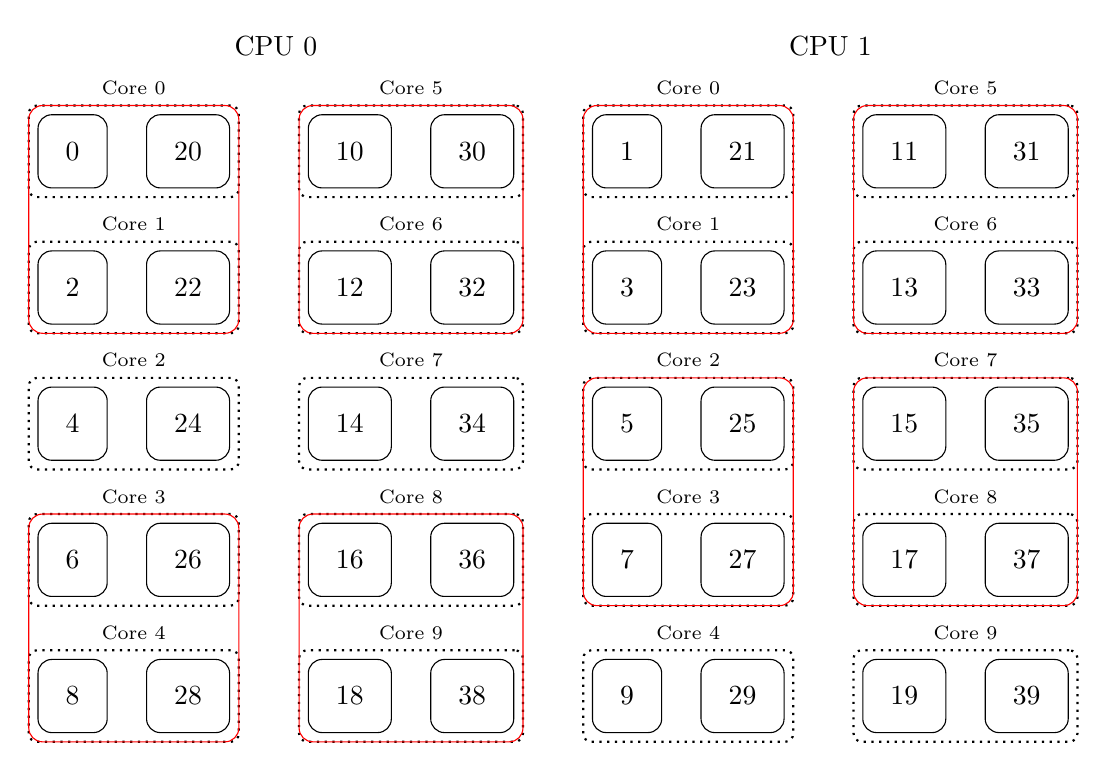
\begin{tikzpicture}[every text node part/.style={align=center}]
\usetikzlibrary{positioning}
\usetikzlibrary{fit}

\tikzstyle{bordered} = [rounded corners=5pt,rectangle,draw,outer sep=0,inner sep=10,minimum size=10]
\tikzstyle{highlight} = [rounded corners=5pt,rectangle,draw=red]
\tikzstyle{rect} = [thick, dotted, rounded corners=3pt]
\tikzstyle{packet} = [draw, ellipse]
\tikzstyle{cable} = [draw=black, line width=1]
\tikzstyle{arrow} = [draw,-latex]

\node [bordered] (0) {0};
\node [bordered, right=of 0, xshift=-.5cm] (20) {20};
\node [draw, rect, fit=(0) (20), label=above:{\scriptsize Core 0}] {};

\node [bordered, below=of 0, yshift=.2cm] (2) {2};
\node [bordered, right=of 2, xshift=-.5cm] (22) {22};
\node [draw, rect, fit=(2) (22), label=above:{\scriptsize Core 1}] {};

\node [highlight, fit=(0) (22)] {};

\node [bordered, below=of 2, yshift=.2cm] (4) {4};
\node [bordered, right=of 4, xshift=-.5cm] (24) {24};
\node [draw, rect, fit=(4) (24), label=above:{\scriptsize Core 2}] {};

\node [bordered, below=of 4, yshift=.2cm] (6) {6};
\node [bordered, right=of 6, xshift=-.5cm] (26) {26};
\node [draw, rect, fit=(6) (26), label=above:{\scriptsize Core 3}] {};

\node [bordered, below=of 6, yshift=.2cm] (8) {8};
\node [bordered, right=of 8, xshift=-.5cm] (28) {28};
\node [draw, rect, fit=(8) (28), label=above:{\scriptsize Core 4}] {};

\node [highlight, fit=(6) (28)] {};

\node [bordered, right=of 20] (10) {10};
\node [bordered, right=of 10, xshift=-.5cm] (30) {30};
\node [draw, rect, fit=(10) (30), label=above:{\scriptsize Core 5}] {};

\node [bordered, below=of 10, yshift=.2cm] (12) {12};
\node [bordered, right=of 12, xshift=-.5cm] (32) {32};
\node [draw, rect, fit=(12) (32), label=above:{\scriptsize Core 6}] {};

\node [highlight, fit=(10) (32)] {};

\node [bordered, below=of 12, yshift=.2cm] (14) {14};
\node [bordered, right=of 14, xshift=-.5cm] (34) {34};
\node [draw, rect, fit=(14) (34), label=above:{\scriptsize Core 7}] {};

\node [bordered, below=of 14, yshift=.2cm] (16) {16};
\node [bordered, right=of 16, xshift=-.5cm] (36) {36};
\node [draw, rect, fit=(16) (36), label=above:{\scriptsize Core 8}] {};

\node [bordered, below=of 16, yshift=.2cm] (18) {18};
\node [bordered, right=of 18, xshift=-.5cm] (38) {38};
\node [draw, rect, fit=(18) (38), label=above:{\scriptsize Core 9}] {};

\node [highlight, fit=(16) (38)] {};


\node [fit=(0) (30), label=above:CPU 0, yshift=.5cm] (cpu0) {};


\node [bordered, right=of 30] (1) {1};
\node [bordered, right=of 1, xshift=-.5cm] (21) {21};
\node [draw, rect, fit=(1) (21), label=above:{\scriptsize Core 0}] {};

\node [bordered, below=of 1, yshift=.2cm] (3) {3};
\node [bordered, right=of 3, xshift=-.5cm] (23) {23};
\node [draw, rect, fit=(3) (23), label=above:{\scriptsize Core 1}] {};

\node [highlight, fit=(1) (23)] {};

\node [bordered, below=of 3, yshift=.2cm] (5) {5};
\node [bordered, right=of 5, xshift=-.5cm] (25) {25};
\node [draw, rect, fit=(5) (25), label=above:{\scriptsize Core 2}] {};

\node [bordered, below=of 5, yshift=.2cm] (7) {7};
\node [bordered, right=of 7, xshift=-.5cm] (27) {27};
\node [draw, rect, fit=(7) (27), label=above:{\scriptsize Core 3}] {};

\node [highlight, fit=(5) (27)] {};

\node [bordered, below=of 7, yshift=.2cm] (9) {9};
\node [bordered, right=of 9, xshift=-.5cm] (29) {29};
\node [draw, rect, fit=(9) (29), label=above:{\scriptsize Core 4}] {};

\node [bordered, right=of 21] (11) {11};
\node [bordered, right=of 11, xshift=-.5cm] (31) {31};
\node [draw, rect, fit=(11) (31), label=above:{\scriptsize Core 5}] {};

\node [bordered, below=of 11, yshift=.2cm] (13) {13};
\node [bordered, right=of 13, xshift=-.5cm] (33) {33};
\node [draw, rect, fit=(13) (33), label=above:{\scriptsize Core 6}] {};

\node [highlight, fit=(11) (33)] {};

\node [bordered, below=of 13, yshift=.2cm] (15) {15};
\node [bordered, right=of 15, xshift=-.5cm] (35) {35};
\node [draw, rect, fit=(15) (35), label=above:{\scriptsize Core 7}] {};

\node [bordered, below=of 15, yshift=.2cm] (17) {17};
\node [bordered, right=of 17, xshift=-.5cm] (37) {37};
\node [draw, rect, fit=(17) (37), label=above:{\scriptsize Core 8}] {};

\node [highlight, fit=(15) (37)] {};

\node [bordered, below=of 17, yshift=.2cm] (19) {19};
\node [bordered, right=of 19, xshift=-.5cm] (39) {39};
\node [draw, rect, fit=(19) (39), label=above:{\scriptsize Core 9}] {};

\node [fit=(1) (31), label=above:CPU 1, yshift=.5cm] (cpu1) {};
\end{tikzpicture}